% Options for packages loaded elsewhere
\PassOptionsToPackage{unicode}{hyperref}
\PassOptionsToPackage{hyphens}{url}
%
\documentclass[
]{frontiersSCNS}
\usepackage{lmodern}
\usepackage{amssymb,amsmath}
\usepackage{ifxetex,ifluatex}
\ifnum 0\ifxetex 1\fi\ifluatex 1\fi=0 % if pdftex
  \usepackage[T1]{fontenc}
  \usepackage[utf8]{inputenc}
  \usepackage{textcomp} % provide euro and other symbols
\else % if luatex or xetex
  \usepackage{unicode-math}
  \defaultfontfeatures{Scale=MatchLowercase}
  \defaultfontfeatures[\rmfamily]{Ligatures=TeX,Scale=1}
\fi
% Use upquote if available, for straight quotes in verbatim environments
\IfFileExists{upquote.sty}{\usepackage{upquote}}{}
\IfFileExists{microtype.sty}{% use microtype if available
  \usepackage[]{microtype}
  \UseMicrotypeSet[protrusion]{basicmath} % disable protrusion for tt fonts
}{}
\makeatletter
\@ifundefined{KOMAClassName}{% if non-KOMA class
  \IfFileExists{parskip.sty}{%
    \usepackage{parskip}
  }{% else
    \setlength{\parindent}{0pt}
    \setlength{\parskip}{6pt plus 2pt minus 1pt}}
}{% if KOMA class
  \KOMAoptions{parskip=half}}
\makeatother
\usepackage{xcolor}
\IfFileExists{xurl.sty}{\usepackage{xurl}}{} % add URL line breaks if available
\IfFileExists{bookmark.sty}{\usepackage{bookmark}}{\usepackage{hyperref}}
\hypersetup{
  pdftitle={Relationships between food groups and eating time slots according to diabetes status in adults from the UK National Diet and Nutrition Survey (2008--2017)},
  hidelinks,
  pdfcreator={LaTeX via pandoc}}
\urlstyle{same} % disable monospaced font for URLs
\usepackage{color}
\usepackage{fancyvrb}
\newcommand{\VerbBar}{|}
\newcommand{\VERB}{\Verb[commandchars=\\\{\}]}
\DefineVerbatimEnvironment{Highlighting}{Verbatim}{commandchars=\\\{\}}
% Add ',fontsize=\small' for more characters per line
\usepackage{framed}
\definecolor{shadecolor}{RGB}{248,248,248}
\newenvironment{Shaded}{\begin{snugshade}}{\end{snugshade}}
\newcommand{\AlertTok}[1]{\textcolor[rgb]{0.94,0.16,0.16}{#1}}
\newcommand{\AnnotationTok}[1]{\textcolor[rgb]{0.56,0.35,0.01}{\textbf{\textit{#1}}}}
\newcommand{\AttributeTok}[1]{\textcolor[rgb]{0.77,0.63,0.00}{#1}}
\newcommand{\BaseNTok}[1]{\textcolor[rgb]{0.00,0.00,0.81}{#1}}
\newcommand{\BuiltInTok}[1]{#1}
\newcommand{\CharTok}[1]{\textcolor[rgb]{0.31,0.60,0.02}{#1}}
\newcommand{\CommentTok}[1]{\textcolor[rgb]{0.56,0.35,0.01}{\textit{#1}}}
\newcommand{\CommentVarTok}[1]{\textcolor[rgb]{0.56,0.35,0.01}{\textbf{\textit{#1}}}}
\newcommand{\ConstantTok}[1]{\textcolor[rgb]{0.00,0.00,0.00}{#1}}
\newcommand{\ControlFlowTok}[1]{\textcolor[rgb]{0.13,0.29,0.53}{\textbf{#1}}}
\newcommand{\DataTypeTok}[1]{\textcolor[rgb]{0.13,0.29,0.53}{#1}}
\newcommand{\DecValTok}[1]{\textcolor[rgb]{0.00,0.00,0.81}{#1}}
\newcommand{\DocumentationTok}[1]{\textcolor[rgb]{0.56,0.35,0.01}{\textbf{\textit{#1}}}}
\newcommand{\ErrorTok}[1]{\textcolor[rgb]{0.64,0.00,0.00}{\textbf{#1}}}
\newcommand{\ExtensionTok}[1]{#1}
\newcommand{\FloatTok}[1]{\textcolor[rgb]{0.00,0.00,0.81}{#1}}
\newcommand{\FunctionTok}[1]{\textcolor[rgb]{0.00,0.00,0.00}{#1}}
\newcommand{\ImportTok}[1]{#1}
\newcommand{\InformationTok}[1]{\textcolor[rgb]{0.56,0.35,0.01}{\textbf{\textit{#1}}}}
\newcommand{\KeywordTok}[1]{\textcolor[rgb]{0.13,0.29,0.53}{\textbf{#1}}}
\newcommand{\NormalTok}[1]{#1}
\newcommand{\OperatorTok}[1]{\textcolor[rgb]{0.81,0.36,0.00}{\textbf{#1}}}
\newcommand{\OtherTok}[1]{\textcolor[rgb]{0.56,0.35,0.01}{#1}}
\newcommand{\PreprocessorTok}[1]{\textcolor[rgb]{0.56,0.35,0.01}{\textit{#1}}}
\newcommand{\RegionMarkerTok}[1]{#1}
\newcommand{\SpecialCharTok}[1]{\textcolor[rgb]{0.00,0.00,0.00}{#1}}
\newcommand{\SpecialStringTok}[1]{\textcolor[rgb]{0.31,0.60,0.02}{#1}}
\newcommand{\StringTok}[1]{\textcolor[rgb]{0.31,0.60,0.02}{#1}}
\newcommand{\VariableTok}[1]{\textcolor[rgb]{0.00,0.00,0.00}{#1}}
\newcommand{\VerbatimStringTok}[1]{\textcolor[rgb]{0.31,0.60,0.02}{#1}}
\newcommand{\WarningTok}[1]{\textcolor[rgb]{0.56,0.35,0.01}{\textbf{\textit{#1}}}}
\usepackage{graphicx,grffile}
\makeatletter
\def\maxwidth{\ifdim\Gin@nat@width>\linewidth\linewidth\else\Gin@nat@width\fi}
\def\maxheight{\ifdim\Gin@nat@height>\textheight\textheight\else\Gin@nat@height\fi}
\makeatother
% Scale images if necessary, so that they will not overflow the page
% margins by default, and it is still possible to overwrite the defaults
% using explicit options in \includegraphics[width, height, ...]{}
\setkeys{Gin}{width=\maxwidth,height=\maxheight,keepaspectratio}
% Set default figure placement to htbp
\makeatletter
\def\fps@figure{htbp}
\makeatother
\setlength{\emergencystretch}{3em} % prevent overfull lines
\providecommand{\tightlist}{%
  \setlength{\itemsep}{0pt}\setlength{\parskip}{0pt}}
\setcounter{secnumdepth}{-\maxdimen} % remove section numbering

\title{Relationships between food groups and eating time slots according to
diabetes status in adults from the UK National Diet and Nutrition Survey
(2008--2017)}
\author{true \and true \and true}
\date{}

\begin{document}
\maketitle

\begin{abstract}

Abstract length and content varies depending on article type. Refer to 
\url{http://www.frontiersin.org/about/AuthorGuidelines} for abstract requirement
and length according to article type.

%All article types: you may provide up to 8 keywords; at least 5 are mandatory.
\tiny
 \keyFont{ \section{Keywords:} Text Text Text Text Text Text Text Text } 

\end{abstract}

\hypertarget{introduction}{%
\section*{Introduction}\label{introduction}}
\addcontentsline{toc}{section}{Introduction}

Cite fancy references ({\textbf{???}}). As demonstrated in
({\textbf{???}}), citations can also be automatically reference.
Multiple references are separated by semicolons ({\textbf{???}};
{\textbf{???}}).

\hypertarget{results}{%
\section*{Results}\label{results}}
\addcontentsline{toc}{section}{Results}

\hypertarget{subsection-1}{%
\subsection*{Subsection 1}\label{subsection-1}}
\addcontentsline{toc}{subsection}{Subsection 1}

You can use \texttt{R} chunks directly to plot graphs.

\begin{Shaded}
\begin{Highlighting}[]
\NormalTok{x <-}\StringTok{ }\DecValTok{0}\OperatorTok{:}\DecValTok{100}
\KeywordTok{set.seed}\NormalTok{(}\DecValTok{999}\NormalTok{)}
\NormalTok{y <-}\StringTok{ }\DecValTok{2} \OperatorTok{*}\StringTok{ }\NormalTok{(x }\OperatorTok{+}\StringTok{ }\KeywordTok{rnorm}\NormalTok{(}\KeywordTok{length}\NormalTok{(x), }\DataTypeTok{sd =} \DecValTok{3}\NormalTok{) }\OperatorTok{+}\StringTok{ }\DecValTok{3}\NormalTok{)}
\KeywordTok{plot}\NormalTok{(x, y)}
\end{Highlighting}
\end{Shaded}

\hypertarget{subsection-2}{%
\subsection*{Subsection 2}\label{subsection-2}}
\addcontentsline{toc}{subsection}{Subsection 2}

Frontiers requires figures to be submitted individually, in the same
order as they are referred to in the manuscript. Figures will then be
automatically embedded at the bottom of the submitted manuscript. Kindly
ensure that each table and figure is mentioned in the text and in
numerical order. Permission must be obtained for use of copyrighted
material from other sources (including the web). Please note that it is
compulsory to follow figure instructions. Figures which are not
according to the guidelines will cause substantial delay during the
production process.

\hypertarget{discussion}{%
\section{Discussion}\label{discussion}}

\hypertarget{disclosureconflict-of-interest-statement}{%
\section*{Disclosure/Conflict-of-Interest
Statement}\label{disclosureconflict-of-interest-statement}}
\addcontentsline{toc}{section}{Disclosure/Conflict-of-Interest
Statement}

The authors declare that the research was conducted in the absence of
any commercial or financial relationships that could be construed as a
potential conflict of interest.

\hypertarget{author-contributions}{%
\section*{Author Contributions}\label{author-contributions}}
\addcontentsline{toc}{section}{Author Contributions}

The statement about the authors and contributors can be up to several
sentences long, describing the tasks of individual authors referred to
by their initials and should be included at the end of the manuscript
before the References section.

\hypertarget{acknowledgments}{%
\section*{Acknowledgments}\label{acknowledgments}}
\addcontentsline{toc}{section}{Acknowledgments}

Funding:

\hypertarget{supplemental-data}{%
\section{Supplemental Data}\label{supplemental-data}}

Supplementary Material should be uploaded separately on submission, if
there are Supplementary Figures, please include the caption in the same
file as the figure. LaTeX Supplementary Material templates can be found
in the Frontiers LaTeX folder

\hypertarget{references}{%
\section{References}\label{references}}

A reference list should be automatically created here. However it won't.
Pandoc will place the list of references at the end of the document
instead. There are no convenient solution for now to force Pandoc to do
otherwise. The easiest way to get around this problem is to edit the
LaTeX file created by Pandoc before compiling it again using the
traditional LaTeX commands.

\hypertarget{figures}{%
\section*{Figures}\label{figures}}
\addcontentsline{toc}{section}{Figures}

\begin{figure}

{\centering 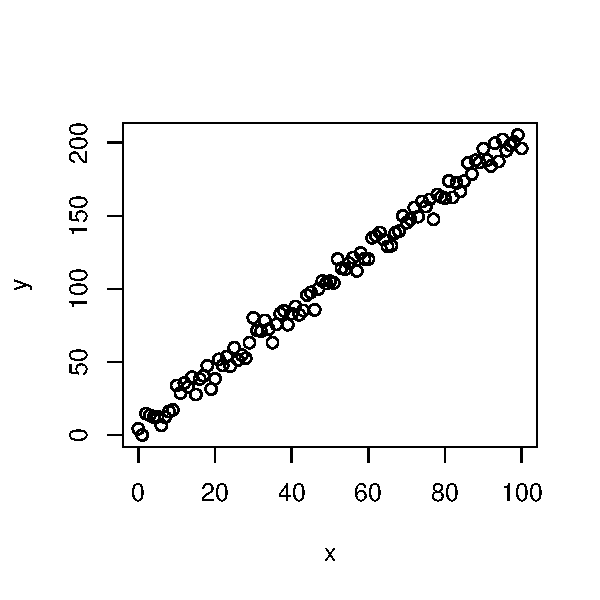
\includegraphics[width=85mm,height=85mm]{manuscriptD_files/figure-latex/Figure-1-1} 

}

\caption{Figure caption}\label{fig:Figure-1}
\end{figure}

\end{document}
